\documentclass[a4paper,10pt]{article}

\usepackage{amsmath}
\usepackage[english]{babel}
\usepackage[style=ieee,backend=bibtex]{biblatex}
	\bibliography{ref.bib}
\usepackage{booktabs}
\usepackage[font={footnotesize}]{caption}
\usepackage[hidelinks]{hyperref}
\usepackage{fancyhdr}
\usepackage{float}
\usepackage{geometry}
\usepackage{graphicx}
\usepackage[latin1]{inputenc}
\usepackage{microtype}
\usepackage{multicol}
\usepackage{multirow}
\usepackage{pgfplots}
	\usepgfplotslibrary{colorbrewer}
	\usepgfplotslibrary{units}
	\pgfplotsset{compat=newest}
	\pgfplotsset{select coords between index/.style 2 args={
	    x filter/.code={
	        \ifnum\coordindex<#1\def\pgfmathresult{}\fi
	        \ifnum\coordindex>#2\def\pgfmathresult{}\fi
	    }
	}}
	\pgfplotsset{cycle list/YlOrRd-9}
\usepackage{placeins}
\usepackage{siunitx}
\usepackage{textcomp}
\usepackage{tikz}
	\usetikzlibrary{arrows}
	\usetikzlibrary{shapes.geometric}
	\usetikzlibrary{positioning}
\usepackage{titling}
\usepackage{threeparttable}
\usepackage{xcolor}
\usepackage{xspace}

\newcommand{\DesignSparkPcb}{DesignSpark
	PCB\textsuperscript{\textregistered}\xspace}
\newcommand{\LTSpice}{LTSpice\textsuperscript{\textregistered}\xspace}

\title{Amplifier Circuit Design in \LTSpice and \DesignSparkPcb}
\author{Z0996690}
\date{\today}

% Headers and footers
\pagestyle{fancy}
\fancyhf{}
\lhead{
\includegraphics[width=0.1\textwidth]{img/Durham.png}}
\chead{\small\thetitle}
\rhead{\theauthor}
\cfoot{\thepage}

\begin{document}

% Title page.
\begin{titlepage}
    \centering
    \vspace*{\fill}
    
\includegraphics[width=0.5\textwidth]{img/Durham.png}\\
    \vspace*{\fill}
    \LARGE\thetitle\\
    \vskip0.2em
    \large Level 3 Electronics and Communication\\
    \vskip0.4em
    \large\theauthor\\
    \vskip0.4em
    \large\thedate\\
    \vspace*{\fill}
\end{titlepage}

\begin{abstract}
	A TI LM386 audio amplifier circuit was designed to drive an \SI{8}{\ohm}
	speaker, with a maximum gain of \SI{35}{\decibel} and maximum bass boost of
	\SI{6}{\decibel} without clipping a \SI{65}{\decibel}SPL input. First the 
	schematic was simulated in \LTSpice to ensure the design met the
	specification. Secondly a layout was formulated using \DesignSparkPcb.
\end{abstract}

\section{Schematic design}

Figure~\ref{fig:blocks} provides an overview of the system the amplifier
circuit was designed for.

\begin{figure}[h]
	\centering
	\begin{footnotesize}
	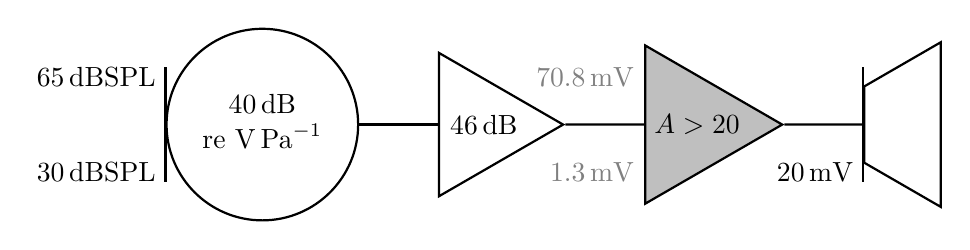
\begin{tikzpicture}
		\node [draw,circle,thick,minimum size=0.15\textwidth]
			(mic) {\begin{tabular}{c}
				\SI{40}{\decibel}\\
				re \si{\volt\per\pascal}
			\end{tabular}};
		% Symbols
		\node [draw,right=of mic,isosceles triangle,minimum width=0.15\textwidth,
			   minimum height=0.1\textwidth,isosceles triangle apex angle=60,
			   thick] (pre) {\SI{46}{\decibel}};
		\node [draw,right=of pre,isosceles triangle,minimum width=0.15\textwidth,
			   minimum height=0.1\textwidth,isosceles triangle apex angle=60,
			   thick,fill=lightgray] (amp) {$A>20$};
		\node [draw,right=of amp,trapezium,shape border rotate=90,thick,
			   minimum size=0.08\textwidth] (speaker) {};

		% Complete mic and loudspeaker
		\draw [thick] ([yshift=0.06\textwidth]mic.west) --
			([yshift=-0.06\textwidth]mic.west);
		\draw [thick] ([yshift=0.06\textwidth]speaker.west) --
			([yshift=-0.06\textwidth]speaker.west);

	   	% System input range.
	   	\node [anchor=east] at ([yshift=0.05\textwidth]mic.west)
	   		{\SI{65}{\decibel}SPL};
	   	\node [anchor=east] at ([yshift=-0.05\textwidth]mic.west)
	   		{\SI{30}{\decibel}SPL};

   		% Amplifier input range.
	   	\node [anchor=east,text=gray] at ([yshift=0.05\textwidth]amp.west)
	   		{\SI{70.8}{\milli\volt}};
	   	\node [anchor=east,text=gray] at ([yshift=-0.05\textwidth]amp.west)
	   		{\SI{1.3}{\milli\volt}};

   		% Speaker input range.
	   	\node [anchor=east] at ([yshift=-0.05\textwidth]speaker.west)
	   		{\SI{20}{\milli\volt}};

   		% Connections
	   	\draw [thick] (mic) -- (pre);
	   	\draw [thick] (pre) -- (amp);
	   	\draw [thick] (amp) -- (speaker);
	\end{tikzpicture}
	\end{footnotesize}
	\caption{System block diagram, indicating minimum and maximum inputs to the
		system and amplifier circuit $A$.}
	\label{fig:blocks}
\end{figure}

The LM386 datasheet described how to implement much of the circuit in
Figure~\ref{fig:ltspice}~\cite{tilm386}. 

Contrary to the datasheet, the schematic included no Boucherot cells as the load
had no inductive component. The DC decoupling capacitors were chosen to be
suitably large to avoid significantly filtering frequencies above
\SI{20}{\hertz}. C2 was originally \SI{2200}{\micro\farad}, but had to be
reduced due to PCB size constraints. The schematic also includes two supply
bypass capacitors to filter noise on the \SI{12}{\volt} line.

\begin{figure}[h]
	\centering
	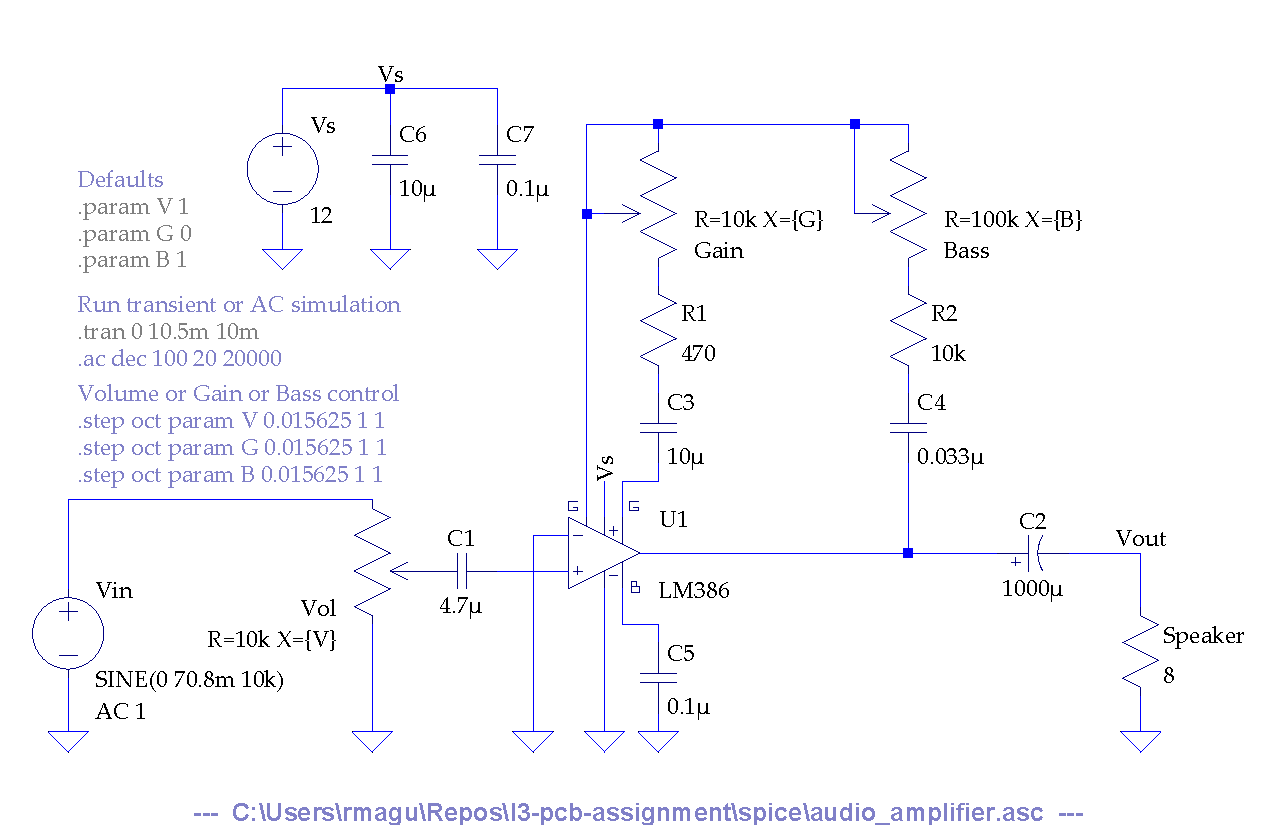
\includegraphics[width=\textwidth]{img/spice_circuit.pdf}
	\caption{Audio amplifier \LTSpice schematic.}
	\label{fig:ltspice}
\end{figure}

A potentiometer provided volume control without distorting the gain response by
attenuating the amplifier input. This can be seen in Figure~\ref{fig:volume}.

\begin{figure}[h]
	\centering
	\begin{footnotesize}
	\begin{tikzpicture}
	    \begin{axis}[
	        xlabel={$f$~/~\si{\hertz}},
	        ylabel={$|A|$~/~\si{\decibel}},
	        xmode = log,
		    enlargelimits=false,
		    enlarge y limits={abs=1},
		    grid=both,
		    grid style={line width=.1pt, draw=gray!10},
		    major grid style={line width=.2pt,draw=gray!50},
		    minor tick num=4,
		    every axis plot/.append style={thick},
		    legend style={font=\tiny,at={(1.01,0.5)},anchor=west},
		    reverse legend,
	    ]
	   		\pgfplotsset{cycle list shift=2}
	        \addplot+[select coords between index={0000}{0300}]
	        	table [x index=0, y index=1]{data/audio_amplifier_vol.txt};
        	\addlegendentry{$2^{-6}$}
	        \addplot+[select coords between index={0301}{0601}]
	        	table [x index=0, y index=1]{data/audio_amplifier_vol.txt};
        	\addlegendentry{$2^{-5}$}
	        \addplot+[select coords between index={0602}{0902}]
	        	table [x index=0, y index=1]{data/audio_amplifier_vol.txt};
        	\addlegendentry{$2^{-4}$}
	        \addplot+[select coords between index={0903}{1203}]
	        	table [x index=0, y index=1]{data/audio_amplifier_vol.txt};
        	\addlegendentry{$2^{-3}$}
	        \addplot+[select coords between index={1204}{1504}]
	        	table [x index=0, y index=1]{data/audio_amplifier_vol.txt};
        	\addlegendentry{$2^{-2}$}
	        \addplot+[select coords between index={1505}{1805}]
	        	table [x index=0, y index=1]{data/audio_amplifier_vol.txt};
        	\addlegendentry{$2^{-1}$}
	        \addplot+[select coords between index={1806}{2106}]
	        	table [x index=0, y index=1]{data/audio_amplifier_vol.txt};
        	\addlegendentry{$1$}
	    \end{axis}
	\end{tikzpicture}
	\end{footnotesize}
	\caption{Bode plot of amplifier gain as volume potentiometer varies
		logarithmically. Set with maximum gain and minimum bass boost.}
	\label{fig:volume}
\end{figure}

In simulation, bypassing pins 1 and 8 with a purely
capacitive load resulted in clipping for the \SI{70.8}{\milli\volt} input.
The \SI{46}{\decibel} maximum gain was limited to \SI{35}{\decibel} by placing
R1 in series with POT2. Varying POT2 varied the gain loop resistance from
\SIrange{470}{10470}{\ohm}, decreasing the gain as indicated in
Figure~\ref{fig:gain}. At \SI{35}{\decibel}, the output was undistorted, as
evidenced by Figure~\ref{fig:clipping}.

\begin{figure}[h]
	\centering
	\begin{footnotesize}
	\begin{tikzpicture}
	    \begin{axis}[
	        xlabel={$f$~/~\si{\hertz}},
	        ylabel={$|A|$~/~\si{\decibel}},
	        xmode = log,
		    enlargelimits=false,
		    enlarge y limits={abs=1},
		    grid=both,
		    grid style={line width=.1pt, draw=gray!10},
		    major grid style={line width=.2pt,draw=gray!50},
		    minor tick num=4,
		    every axis plot/.append style={thick},
		    legend style={font=\tiny,at={(1.01,0.5)},anchor=west},
		    reverse legend,
	    ]
	   		\pgfplotsset{cycle list shift=1}
	        \addplot+[select coords between index={1806}{2106}]
	        	table [x index=0, y index=1]{data/audio_amplifier_vol.txt};
        	\addlegendentry{$0$}
	        \addplot+[select coords between index={0000}{0300}]
	        	table [x index=0, y index=1]{data/audio_amplifier_gain.txt};
        	\addlegendentry{$2^{-6}$}
	        \addplot+[select coords between index={0301}{0601}]
	        	table [x index=0, y index=1]{data/audio_amplifier_gain.txt};
        	\addlegendentry{$2^{-5}$}
	        \addplot+[select coords between index={0602}{0902}]
	        	table [x index=0, y index=1]{data/audio_amplifier_gain.txt};
        	\addlegendentry{$2^{-4}$}
	        \addplot+[select coords between index={0903}{1203}]
	        	table [x index=0, y index=1]{data/audio_amplifier_gain.txt};
        	\addlegendentry{$2^{-3}$}
	        \addplot+[select coords between index={1204}{1504}]
	        	table [x index=0, y index=1]{data/audio_amplifier_gain.txt};
        	\addlegendentry{$2^{-2}$}
	        \addplot+[select coords between index={1505}{1805}]
	        	table [x index=0, y index=1]{data/audio_amplifier_gain.txt};
        	\addlegendentry{$2^{-1}$}
	        \addplot+[select coords between index={1806}{2106}]
	        	table [x index=0, y index=1]{data/audio_amplifier_gain.txt};
        	\addlegendentry{$1$}
	    \end{axis}
	\end{tikzpicture}
	\end{footnotesize}
	\caption{Bode plot of amplifier gain as gain potentiometer varies
		logarithmically. Set with maximum volume and minimum bass boost.}
	\label{fig:gain}
\end{figure}

\begin{figure}[h]
	\centering
	\begin{footnotesize}
	\begin{tikzpicture}
	    \begin{axis}[
	        xlabel={$t$~/~\si{\milli\second}},
	        ylabel={$V_{out}$~/~\si{\volt}},
			change x base=true, x SI prefix=milli,
		    enlargelimits=false,
		    ymin=-4, ymax=4,
		    grid=both,
		    grid style={line width=.1pt, draw=gray!10},
		    major grid style={line width=.2pt,draw=gray!50},
		    minor tick num=4,
		    every axis plot/.append style={thick},
	    ]
	   		\pgfplotsset{cycle list shift=8}
	        \addplot+[select coords between index={1}{383}]
	        	table [x index=0, y index=1]{data/audio_amplifier_trans.txt};
	    \end{axis}
	\end{tikzpicture}
	\end{footnotesize}
	\caption{Maximum output voltage across speaker in response to the maximum
		input voltage---\SI{65}{\decibel}SPL, \SI{10}{\kilo\hertz}.}
	\label{fig:clipping}
\end{figure}

The datasheet describes how a \SI{10}{\kilo\ohm} resistor is required to boost
bass by \SI{6}{\decibel}. In simulation, increasing the series resistance
reduced this effect. A \SI{100}{\kilo\ohm} potentiometer was sufficient to 
effectively open circuit the bass boost branch. Figure~\ref{fig:bass} illustrates 
the \SIrange{0}{6}{\decibel} boost at \SI{80}{\hertz}.

\begin{figure}[h]
	\centering
	\begin{footnotesize}
	\begin{tikzpicture}
	    \begin{axis}[
	        xlabel={$f$~/~\si{\hertz}},
	        ylabel={$|A|$~/~\si{\decibel}},
	        xmode = log,
		    enlargelimits=false,
		    enlarge y limits={abs=1},
		    grid=both,
		    grid style={line width=.1pt, draw=gray!10},
		    major grid style={line width=.2pt,draw=gray!50},
		    minor tick num=4,
		    every axis plot/.append style={thick},
		    legend style={font=\tiny,at={(1.01,0.5)},anchor=west},
		    reverse legend,
	    ]
	   		\pgfplotsset{cycle list shift=2}
	        \addplot+[select coords between index={0000}{0300}]
	        	table [x index=0, y index=1]{data/audio_amplifier_bass.txt};
        	\addlegendentry{$2^{-6}$}
	        \addplot+[select coords between index={0301}{0601}]
	        	table [x index=0, y index=1]{data/audio_amplifier_bass.txt};
        	\addlegendentry{$2^{-5}$}
	        \addplot+[select coords between index={0602}{0902}]
	        	table [x index=0, y index=1]{data/audio_amplifier_bass.txt};
        	\addlegendentry{$2^{-4}$}
	        \addplot+[select coords between index={0903}{1203}]
	        	table [x index=0, y index=1]{data/audio_amplifier_bass.txt};
        	\addlegendentry{$2^{-3}$}
	        \addplot+[select coords between index={1204}{1504}]
	        	table [x index=0, y index=1]{data/audio_amplifier_bass.txt};
        	\addlegendentry{$2^{-2}$}
	        \addplot+[select coords between index={1505}{1805}]
	        	table [x index=0, y index=1]{data/audio_amplifier_bass.txt};
        	\addlegendentry{$2^{-1}$}
	        \addplot+[select coords between index={1806}{2106}]
	        	table [x index=0, y index=1]{data/audio_amplifier_bass.txt};
        	\addlegendentry{1}
	    \end{axis}
	\end{tikzpicture}
	\end{footnotesize}
	\caption{Bode plot of amplifier gain as bass boost potentiometer varies
		logarithmically. Set with maximum volume and gain.}
	\label{fig:bass}
\end{figure}

\FloatBarrier
\section{PCB design}

Table~\ref{tab:bom} lists the components used to implement the schematic. A
large package was used for the input decoupling capacitor to mitigate the 
capacitance change in X7R capacitors subjected to DC biases. A C0G capacitor was
used for the bass boost capacitor, as simulations showed the voltage across this 
component varied wildly and C0G capacitors have no DC response.

\begin{table}[h]
	\centering
	\caption{Bill of materials.}
	\label{tab:bom}
	\begin{footnotesize}
	\begin{tabular}{@{}cr@{, }r@{, }lccc@{}
	}
	\toprule
	Ref &
	\multicolumn{3}{c}{Description} &
	Package &
	Manufacturer number &
	RS number \\
	\midrule
	C1 & \SI{4.7}{\micro\farad} & \SI{25}{\volt} & X7R cap & 1210 &
		KEMET C1210C475K3RACTU & 691-1256 \\
	C2 & \SI{1000}{\micro\farad} & \SI{25}{\volt} & Al cap & FK--H &
		Panasonic EEVF1KE102Q & 708-3434 \\
	C3 & \SI{10}{\micro\farad} & \SI{10}{\volt} & X7R cap & 0805 &
		KEMET C0805C106K8RACTU & 802-9854 \\
	C4 & \SI{0.033}{\micro\farad} & \SI{25}{\volt} & C0G cap & 0805 &
		KEMET C0805C333J3GACTU & (\emph{Farnell}) \\
	C5,7 & \SI{0.1}{\micro\farad} & \SI{25}{\volt} & X7R cap & 0603 &
		KEMET C0603C104J3RACTU & 801-5237 \\
	C6 & \SI{10}{\micro\farad} & \SI{25}{\volt} & X7R cap & 1206 &
		KEMET C1206C104K3RACTU & 802-9977 \\
	JACK1 & \SI{3.5}{\milli\meter} & \multicolumn{2}{@{}l}{stereo jack} & thru &
		Swithcraft 35RAPC2BV4 & (\emph{Farnell}) \\
	POT1,2 & \SI{10}{\kilo\ohm} & \multicolumn{2}{@{}l}{logarithmic pot} & thru &
		Bourns 91A1A-B28-D15L & 522-5153 \\
	POT3 & \SI{100}{\kilo\ohm} & \multicolumn{2}{@{}l}{logarithmic pot} & thru &
		Bourns 91A1A-B28-D20L & 522-5175 \\
	R1 & \SI{470}{\ohm} & \SI{50}{\volt} & resistor & 0603 &
		Panasonic ERJPA3F4700V & 826-6966 \\
	R2 & \SI{10}{\kilo\ohm} & \SI{50}{\volt} & resistor & 0603 &
		Panasonic ERJPA3F1002V & 826-6704 \\
	U1 & \multicolumn{3}{c}{LM386 audio amplifier} & SOIC &
		TI LM386M-1/NOPB & 536-1366 \\
	\bottomrule
	\end{tabular}
	\end{footnotesize}
\end{table}

Custom PCB symbols were created for the Panasonic FK-series size-H
package~\cite{panasonicfk}; the stereo jack~\cite{switchcraft35rapc} and the 
potentiometers~\cite{bourns91_95}.

% \begin{figure}[h]
% 	\centering
% 	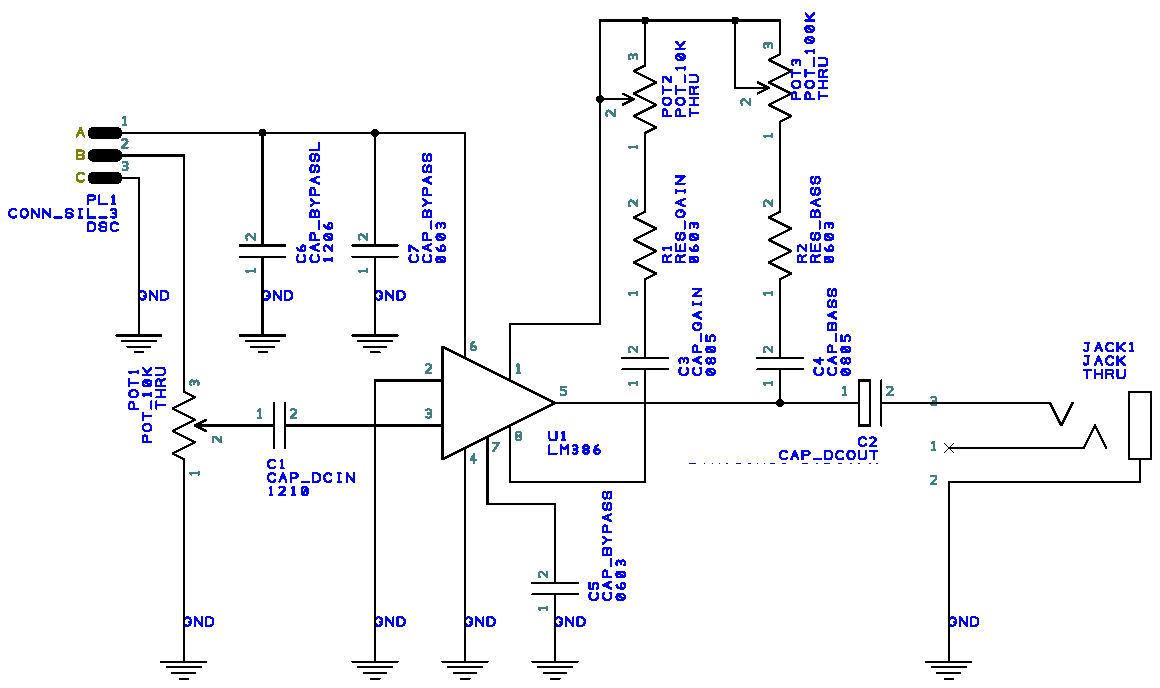
\includegraphics[width=\textwidth]{img/audio_amplifier_sch.pdf}
% 	\caption{Audio amplifier \DesignSparkPcb schematic.}
% \end{figure}

To ensure all traces were sufficiently wide, the maximum current through each
branch was simulated. The trace widths are listed in
Table~\ref{tab:width}. \SI{10}{mil} was the nominal width, whilst
\SI{15}{mil} was for the supply, ground and output traces to minimise voltage
drop. These can be seen in Figure~\ref{fig:pcb}.

\begin{table}[h]
	\centering
	\caption{Trace width calculations due to maximum current with 25 V
		     supply, \SI{1}{oz\per ft^2} trace, \SI{10}{\celsius} temperature
		     rise at \SI{25}{\celsius}.}
    \label{tab:width}
    \begin{footnotesize}
	\begin{tabular}{@{}crrc@{}}
	\toprule
	Branch &
	{$f_{I_{\text{max}}}$ / \si{\hertz}} &
	{$I_{max}$ / \si{\milli\ampere}} &
	Width / mil \\
	\midrule
	Vs   &    85 & 470 & 4.2 \\
	Vin  &    33 &   0 & 0.0 \\
	C1   &    24 &   0 & 0.0 \\
	C2   &    85 & 500 & 4.6 \\ 
	C3   & 20000 & 110 & 0.5 \\
	C4   & 20000 & 170 & 1.0 \\
	C5   & 20000 &   0 & 0.0 \\
	C6   & 20000 &   0 & 0.0 \\
	C7   & 20000 &   0 & 0.0 \\
	U1.1 & 20000 &  65 & 0.3 \\
	\bottomrule
	\end{tabular}
    \end{footnotesize}
\end{table}

\begin{figure}
	\centering
	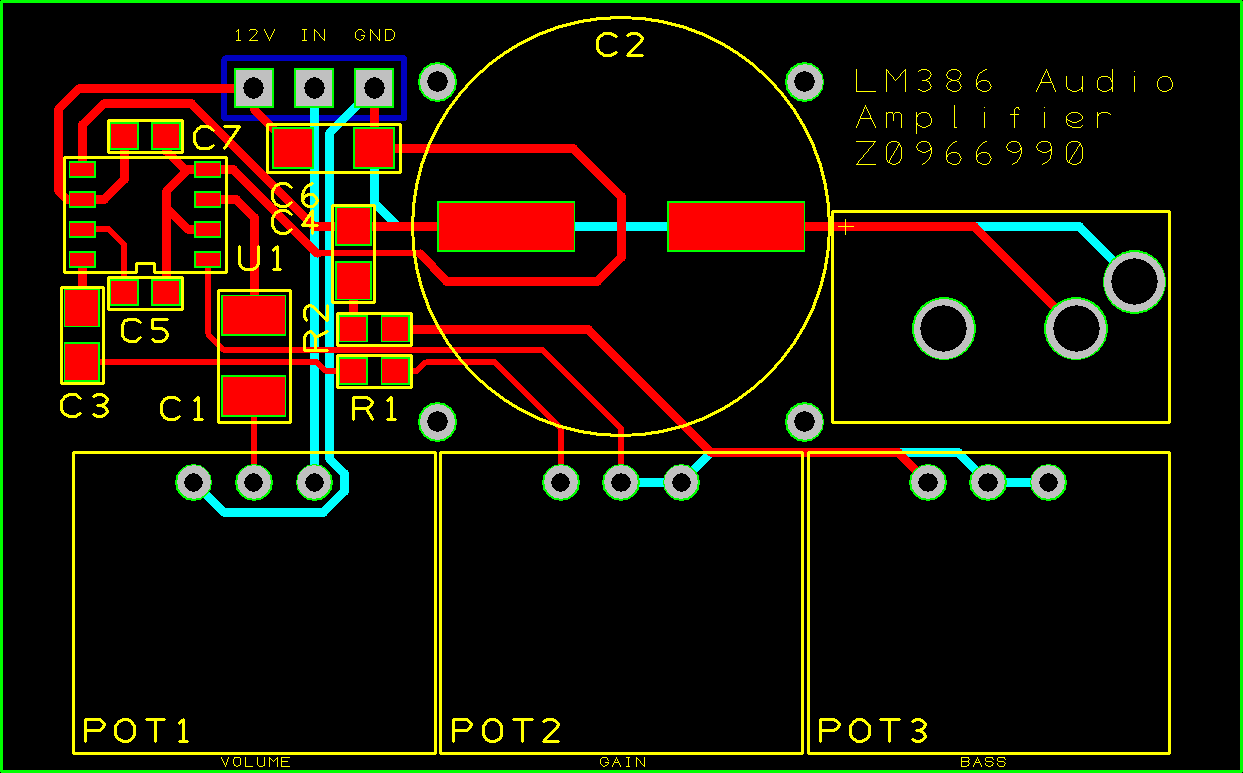
\includegraphics[width=\textwidth]{img/audio_amplifier_pcb.png}
	\caption{Audio amplifier \DesignSparkPcb layout.}
	\label{fig:pcb}
\end{figure}

The larger bypass capacitor C6 was placed as close to the supply as
possible, whilst bypass capacitors C5 and C7 were placed close to the
LM386. The input, output and LM386 were each given their own ground to limit 
interference. The input and output return paths follow the outward path on the 
other side of the board and the gain and bass boost loops were also minimised.

The board was optimised for size and number of vias: measuring 2060 by 1280 mil,
with 0 vias.

\FloatBarrier
\printbibliography

\end{document}